\documentclass[12pt]{article}
\usepackage{tempora}
\usepackage[utf8]{inputenc}
\usepackage[T2A]{fontenc}
\usepackage{cmap}
\usepackage{mathtext}
\usepackage{array}
\usepackage{booktabs}
\usepackage{multirow}
\usepackage[english,russian]{babel}

\usepackage{amsmath,amsfonts,amssymb,amsthm,mathtools} % AMS
\usepackage{icomma}

\usepackage[left=10mm, top=20mm, right=18mm, bottom=15mm, footskip=10mm]{geometry}
\usepackage{indentfirst}
\usepackage{euscript}
\usepackage{mathrsfs}

\usepackage[italicdiff]{physics}
\usepackage{graphicx}
\graphicspath{{images/}}
\DeclareGraphicsExtensions{.pdf,.png,.jpg}
\usepackage{wrapfig}
\usepackage{subcaption}
\usepackage{caption}
\usepackage{float}
\usepackage{fancyvrb}
\usepackage{hyperref}
\usepackage[rgb]{xcolor}

\hypersetup{
    colorlinks=true,
    urlcolor=blue,
    linkcolor=black
}
\captionsetup[figure]{name=Рисунок}
\captionsetup[table]{name=Таблица}
\DeclareUnicodeCharacter{03C9}{\ensuremath{\omega}}

\sloppy
\setlength{\parindent}{1.25cm}

\begin{document}

\thispagestyle{empty}

\begin{center}

\large
Министерство науки и высшего образования Российской Федерации \\
\large
ФЕДЕРАЛЬНОЕ ГОСУДАРСТВЕННОЕ АВТОНОМНОЕ \\
ОБРАЗОВАТЕЛЬНОЕ УЧРЕЖДЕНИЕ ВЫСШЕГО ОБРАЗОВАНИЯ \\
\large
«МОСКОВСКИЙ ФИЗИКО-ТЕХНИЧЕСКИЙ ИНСТИТУТ \\
(НАЦИОНАЛЬНЫЙ ИССЛЕДОВАТЕЛЬСКИЙ УНИВЕРСИТЕТ)» \\
(МФТИ, Физтех)

\vspace{2.5cm}

% \large
% КАФЕДРА ВЫЧИСЛИТЕЛЬНОЙ ФИЗИКИ

% \vspace{0.5cm}

\large
Курс «Вычислительная математика»

\vspace{0.5cm}

\Large
ОТЧЕТ \\
ПО ЛАБОРАТОРНОЙ РАБОТЕ 1

\vspace{0.7cm}

\Large
\textbf{Итерационные методы решения разреженных систем линейных алгебраических уравнений и предобуславливание}

\vspace{0.5cm}

\large
Вариант E4 (электростатика)

\vfill

\vspace{1.5cm}

\large

\noindent
Работу выполнил \hfill  \underline{\hspace{4.2cm}\text{Воронин Денис Б04-407}} \\
\hfill {\hspace{1.6cm} (Ф.И.О., группа)}\par

\vspace{2.5cm}

\noindent
Работу принял, оценка \hfill \underline{\hspace{6cm}} \\
\hfill {\small (подпись, дата, оценка)}

\vfill

Долгопрудный 2026

\end{center}

\newpage

\thispagestyle{empty}
\renewcommand{\contentsname}{ОГЛАВЛЕНИЕ}
\tableofcontents

\newpage

\section{Цель работы}

1. Научиться формировать разреженную матрицу СЛАУ по заданной расчётной формуле (вариант E4, электростатика), хранить её в формате CSR и проверять её структуру, симметричность и положительную определённость.\par

2. Реализовать методы Якоби, Зейделя, последовательной верхней релаксации (ПВР), сопряжённых градиентов (CG) и предобусловленный метод сопряжённых градиентов (PCG) с диагональным и SSOR-предобуславливателями без формирования плотных матриц.\par

3. Сравнить методы по числу итераций, числу умножений матрицы на вектор, времени и памяти; исследовать влияние размера сетки, обусловленности матрицы и предобуславливания; различить невязку и погрешность решения СЛАУ.\par

4. Подтвердить решение независимыми решателями и интерпретировать результат в терминах электростатики.\par

\section{Теоретические сведения}

\subsection{Постановка задачи варианта E4}

В безразмерных переменных решается краевая задача
\[
-\nabla\cdot\bigl(a(x,y)\nabla u\bigr)+c(x,y)\,u=f(x,y),\quad (x,y)\in\Omega=(0,1)^2,\qquad u\big|_{\partial\Omega}=g,
\]
которая для варианта E4 имеет коэффициенты
\[
a(x,y)=1{,}5+3\,G_{0{,}30;\,0{,}70;\,0{,}15}(x,y),\qquad c\equiv0,\qquad f(x,y)=12\sin(\pi x)\sin(\pi y),\qquad g\equiv0,
\]
\[
G_{x_0,y_0,\sigma}(x,y)=\exp\left(-\frac{(x-x_0)^2+(y-y_0)^2}{2\sigma^2}\right).
\]
Здесь $u$~--- электростатический потенциал, $a$~--- диэлектрическая проницаемость (гладкое включение повышенной проницаемости с центром в точке $(0{,}3;\,0{,}7)$, $1{,}5\le a\le4{,}5$), $f$~--- плотность объёмного заряда (максимум в центре области), граница заземлена (электроды). Матрица $A$ и правая часть $b$ строятся по формуле (3) методических указаний на сетке $N\times N$ узлов ($h=1/(N-1)$), число неизвестных $n=(N-2)^2$, нумерация $m=(i-1)+(j-1)(N-2)$. В каждой строке не более пяти ненулевых элементов, $A=A^T$, $A>0$ (формула (4) методических указаний). Матрица хранится в формате CSR (массивы \texttt{data}, \texttt{indices}, \texttt{indptr}); память равна $12\,\mathrm{nnz}+4(n+1)$ байт. Плотная матрица формируется только для проверок на сетке $N=8$. Погрешность дискретизации исходной краевой задачи в работе не оценивается.

\subsection{Реализованные методы}

Все методы реализованы самостоятельно (библиотечные решатели использованы только на этапе 4).\par

\textbf{Стационарные методы.} Метод Якоби, метод Зейделя и ПВР реализованы по формулам (7), (9) и (11) методических указаний с построчным обходом CSR-структуры. Начальное приближение $x^{(0)}=0$. На каждой итерации вычисляется \emph{истинная} нормированная невязка $\eta_s=\|b-Ax^{(s)}\|_2/\|b\|_2$. Одна итерация стоит $O(\mathrm{nnz})$; в столбце «Матвекс» для стационарных методов указано число итераций (дополнительный матвек, вычисляющий $\eta_s$, не учитывается).\par

\textbf{CG} реализован по формулам (12), \textbf{PCG}~--- по псевдокоду п.\,6.4 методических указаний. Невязка обновляется рекуррентно, а при $s=0,50,100,\dots$ заменяется явно вычисленной $b-Ax^{(s)}$ (борьба с накоплением погрешностей округления); эти дополнительные умножения входят в счётчик «Матвекс». На каждой итерации проверяются условия $(p^{(s)})^TAp^{(s)}>0$ и $(r^{(s)})^Tz^{(s)}>0$, при нарушении выполнение прерывается.\par

\textbf{Предобуславливатели.} Диагональный: $P=D=\mathrm{diag}(A)$, $z_i=r_i/a_{ii}$. SSOR:
\[
P_\text{SSOR}=\frac{1}{\omega(2-\omega)}\,(D+\omega L)\,D^{-1}\,(D+\omega L^T),
\]
действие $P_\text{SSOR}^{-1}$ на вектор выполняется двумя разреженными треугольными подстановками: $By=r$, $B^Tz_0=Dy$, $z=\omega(2-\omega)z_0$, где $B=D+\omega L$ (функция \texttt{spsolve\_triangular}); матрицы $B$, $B^T$ формируются один раз (время $t_\text{подг}$), обратные матрицы не формируются. Допустимость в PCG: $P_D$ симметрична и положительно определена, так как $a_{mm}>0$; $P_\text{SSOR}=CC^T$ с невырожденной нижней треугольной $C=(D+\omega L)D^{-1/2}/\sqrt{\omega(2-\omega)}$ при $0<\omega<2$, поэтому $P_\text{SSOR}=P_\text{SSOR}^T>0$. На малой матрице ($N=8$, $\omega=1{,}5$) это проверено численно: $\|P-P^T\|/\|P\|=$ $4{,}97\cdot10^{-17}$, $\lambda_{\min}(P_\text{SSOR})=$ 61{,}45.\par

\subsection{Критерий остановки и обозначения}

Во всех методах: $\eta_s\le\varepsilon_{res}=10^{-8}$, максимум 10\,000 итераций; достижение максимума фиксируется как \emph{недостижение порога}. В таблицах указано именно истинное значение $\eta$, пересчитанное независимо от решателя по найденному $x$. Погрешность решения СЛАУ $\delta_s=\|u^*-x^{(s)}\|_2/\|u^*\|_2$ связана с невязкой оценкой $\delta_s\le\mu(A)\,\eta_s$.\par

\subsection{Спектральные оценки, используемые при анализе}

Собственные числа $\lambda_{\min}$, $\lambda_{\max}$ матриц $A$ и $D^{-1/2}AD^{-1/2}$ найдены разреженным методом Ланцоша (\texttt{scipy.sparse.linalg.eigsh}, для $\lambda_{\min}$~--- со сдвигом $\sigma=0$), без плотных матриц; $\mu(A)=\lambda_{\max}/\lambda_{\min}$. Собственные числа $D^{-1}A$ равны $\lambda_i$, матрица перехода Якоби $R_J=I-D^{-1}A$ имеет $\rho(R_J)=\max(1-\lambda_{\min},\lambda_{\max}-1)$. Для матрицы (3) в естественной нумерации (двухцветное упорядочение по чётности $i+j$) $\rho(R_{GS})=\rho(R_J)^2$,
\[
\omega_{opt}=\frac{2}{1+\sqrt{1-\rho(R_J)^2}},\qquad \rho(R_{SOR}(\omega_{opt}))=\omega_{opt}-1,\qquad k\approx\frac{\ln(1/\varepsilon_{res})}{\ln(1/\rho)}.
\]
Для CG и PCG числа итераций оцениваются через $\kappa$ по классической оценке $s\lesssim\frac12\sqrt{\kappa}\ln(2/\varepsilon)$. Эффективное число обусловленности $\kappa(P_\text{SSOR}^{-1}A)$ оценивается по крайним числам Ритца матрицы Ланцоша, построенной по коэффициентам $\alpha_s,\beta_s$ самого PCG; метод проверен на CG, где крайние числа Ритца совпадают с $\lambda_{\min},\lambda_{\max}$ из \texttt{eigsh} (относительное расхождение $\lambda_{\max}$ при $N=128$: $1{,}1\cdot10^{-12}$).\par

\section{Ход работы}

Все числа, таблицы и графики получены программой, полный текст которой приведён в приложении Б; результаты записаны в файл \texttt{results\_all\_stages.csv} (столбцы: $N$, метод, $n$, nnz, итерации, матвеки, статус сходимости, $t_\text{подг}$, $t_\text{итер}$, $\eta$, $\varepsilon_{res}$, память CSR). Расчёты выполнены в арифметике двойной точности, Python 3.12.3, NumPy 2.4.4, SciPy 1.17.1 (один вычислительный поток).

\subsection{Этап 1. Проверка сборки матрицы ($N=8$)}

На сетке $N=8$ получена матрица $36\times36$ (рис.~\ref{fig:spy}). Результаты проверок приведены в таблице~\ref{tab:stage1}.\par

\begin{table}[H]
\centering
\caption{Результаты проверки сборки матрицы на сетке $N=8$}
\label{tab:stage1}
\small
\begin{tabular}{|l|c|}
\hline
Проверка & Результат \\
\hline
Размер матрицы $A$ & $36\times36$ (внутренних узлов $6\times6$) \\
Число ненулевых элементов $\mathrm{nnz}(A)$ & 156 (оценка $\le5n=180$) \\
Максимум ненулевых в строке & 5 \\
$\|A-A^{T}\|_F/\|A\|_F$ & $0$ \\
Диагональные элементы $a_{mm}$ & от 294,00 до 771,23 ($>0$) \\
$z^{T}Az$, $z=(1,\dots,1)$ & 2024,66 \\
$z^{T}Az$, $z_k=(-1)^k$ & 14048,26 \\
$z^{T}Az$, $z_k=\sin(\pi k/n)$ & 945,01 \\
Разложение Холецкого без сдвига & выполнено \\
Собственные числа $A$ (плотный расчёт, только $N=8$) & $\lambda_{\min}=35{,}21$, $\lambda_{\max}=1168{,}3$ \\
$\|Au-\mathcal{A}u\|/\|Au\|$ (независимая реализация формулы (3)) & $7{,}85\cdot10^{-17}$ \\
\hline
\end{tabular}
\end{table}

\begin{figure}[H]
    \centering
    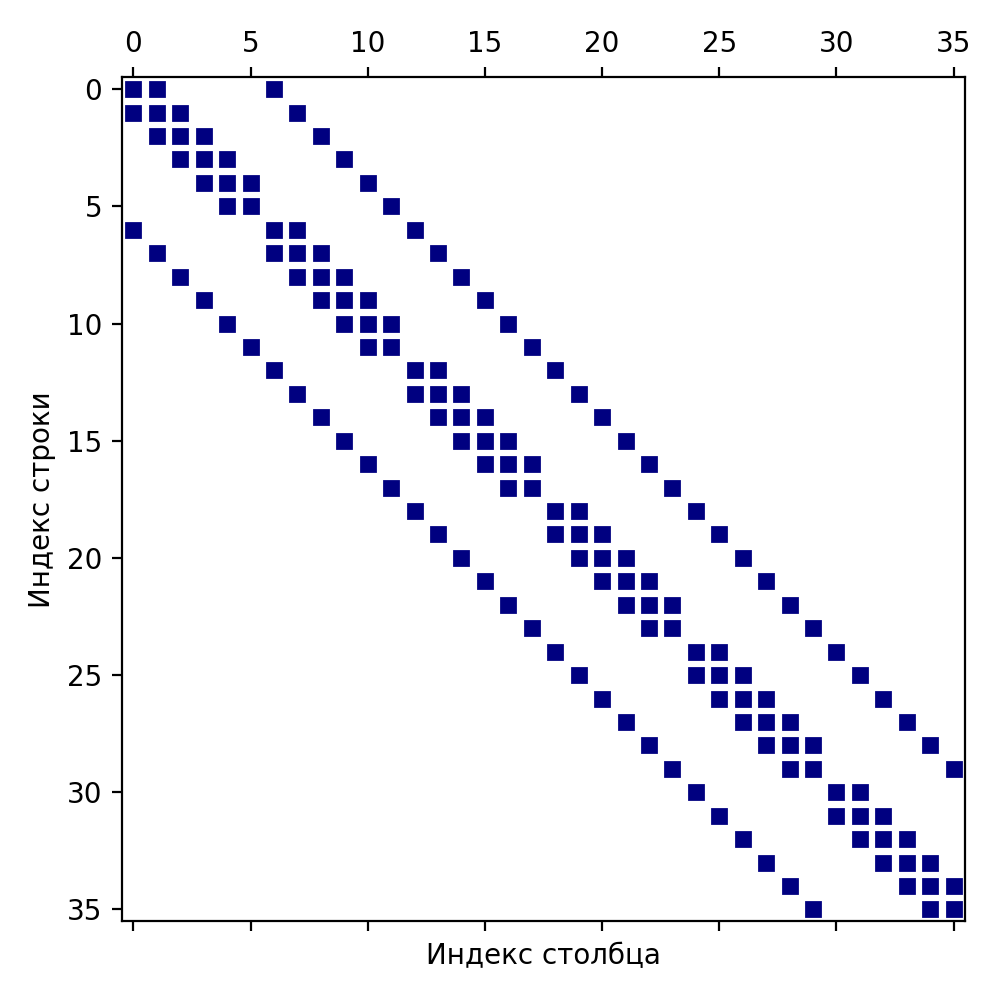
\includegraphics[width=7.5cm]{fig_spy_N8.png}
    \caption{Портрет матрицы $A$ ($N=8$, $\mathrm{nnz}=156$)}
    \label{fig:spy}
\end{figure}

Строка $m=0$ соответствует узлу $(i,j)=(1,1)$, два соседа которого (слева и снизу) лежат на границе с $g=0$, поэтому их вклад в правую часть равен нулю и в строке остаются три элемента; уравнение:
\[
295{,}1928\,u_{11}-73{,}6168\,u_{21}-74{,}4795\,u_{12}=2{,}2591,
\]
где $b_0=f(1/7,1/7)=12\sin^2(\pi/7)$. Число ненулевых элементов $156=5n-4(N-2)=180-24$: у узлов, примыкающих к границе, не хватает связей с граничными соседями. Независимая векторизованная реализация формулы (3) (без построения матрицы) совпадает с $Au$ до $10^{-16}$, что подтверждает правильность индексации и коэффициентов связи. Матрица симметрична с точностью до округления, диагональ положительна, $z^TAz>0$ для всех тестовых векторов, разложение Холецкого без диагонального сдвига выполняется и все собственные числа положительны. \textbf{Этап выполнен.}

\subsection{Этап 2. Стационарные методы}

\textbf{Проверка на системе с известным решением.} На сетке $N=32$ ($n=900$) задано $u^*_m=1+\sin(2\pi m/n)+0{,}1\cos(6\pi m/n)$, $b^*=Au^*$. Результаты в таблице~\ref{tab:test_stat}; в расчёте для ПВР использовано $\omega=1{,}92$ (подбор ниже).\par

\begin{table}[H]
\centering
\caption{Тестовая система ($N=32$, $b^*=Au^*$, $x^{(0)}=0$, порог $\varepsilon_{res}=10^{-8}$): невязка и погрешность стационарных методов; $\mu(A)=887{,}6$}
\label{tab:test_stat}
\small
\begin{tabular}{|l|c|c|c|c|c|}
\hline
Метод & Итераций & $\eta_s$ & $\delta_s$ & $\delta_s/\eta_s$ & $\mu(A)\,\eta_s$ \\
\hline
Якоби & 3397 & $1{,}00\cdot10^{-8}$ & $1{,}36\cdot10^{-7}$ & 13,64 & $8{,}87\cdot10^{-6}$ \\
Зейдель & 1694 & $9{,}91\cdot10^{-9}$ & $1{,}35\cdot10^{-7}$ & 13,60 & $8{,}80\cdot10^{-6}$ \\
ПВР ($\omega$=1,920) & 241 & $9{,}33\cdot10^{-9}$ & $1{,}17\cdot10^{-9}$ & 0,13 & $8{,}28\cdot10^{-6}$ \\
\hline
\end{tabular}
\end{table}

Все три метода достигли порога $\varepsilon_{res}=10^{-8}$. Отношение $\delta_s/\eta_s$ для методов Якоби и Зейделя равно 13,6, для ПВР~--- 0,13. Оценка $\delta_s\le\mu(A)\eta_s$ ($\mu(A)=887{,}6$) выполняется с большим запасом: она достижима лишь тогда, когда невязка целиком направлена по собственному вектору, отвечающему $\lambda_{\min}$. Основная мысль таблицы~--- малая невязка сама по себе не определяет погрешность: у стационарных методов ошибка накапливается в гладких (медленно затухающих) компонентах, поэтому при одной и той же $\eta_s\approx10^{-8}$ их погрешность на два порядка больше, чем у ПВР, и она может быть в $\mu(A)$ раз больше невязки.\par

\textbf{Подбор $\omega$ для ПВР.} На сетке $N=64$ (задача варианта) исследовано 10 значений $\omega\in[1;\,1{,}95]$ и затем 15 значений на отрезке $[1{,}85;\,1{,}99]$ (таблица~\ref{tab:sorscan}, рис.~\ref{fig:omega}, слева). Наилучшее среди проверенных значение: $\omega=1{,}92$ (253 итераций). Оно близко к теоретическому $\omega_{opt}=1{,}911$, вычисленному по $\rho(R_J)$ (таблица~\ref{tab:spec}), но теоретически оптимальным не называется: поиск дискретен. Минимум несимметричен: при $\omega>\omega_{opt}$ радиус сходимости равен $\omega-1$ и число итераций резко растёт ($\omega=1{,}99$ требует более 2\,000 итераций), поэтому при выборе $\omega$ безопаснее ошибиться в меньшую сторону.\par

\begin{table}[H]
\centering
\caption{Подбор параметра $\omega$ метода ПВР на сетке $N=64$ (число итераций до $\eta_s\le10^{-8}$)}
\label{tab:sorscan}
\small
\begin{tabular}{|c|c|c|c|}
\hline
\multicolumn{2}{|c|}{Грубый поиск} & \multicolumn{2}{|c|}{Уточнение} \\
\hline
$\omega$ & Итераций & $\omega$ & Итераций \\ \hline
$1{,}000$ & $8577$ & $1{,}85$ & $645$ \\
$1{,}106$ & $6938$ & $1{,}86$ & $590$ \\
$1{,}211$ & $5584$ & $1{,}87$ & $534$ \\
$1{,}317$ & $4446$ & $1{,}88$ & $477$ \\
$1{,}422$ & $3477$ & $1{,}89$ & $418$ \\
$1{,}528$ & $2640$ & $1{,}90$ & $353$ \\
$1{,}633$ & $1910$ & $1{,}91$ & $269$ \\
$1{,}739$ & $1263$ & $1{,}92$ & $253$ \\
$1{,}844$ & $675$ & $1{,}93$ & $288$ \\
$1{,}950$ & $399$ & $1{,}94$ & $349$ \\
 &  & $1{,}95$ & $399$ \\
 &  & $1{,}96$ & $505$ \\
 &  & $1{,}97$ & $676$ \\
 &  & $1{,}98$ & $1009$ \\
 &  & $1{,}99$ & $2035$ \\
\hline
\end{tabular}
\end{table}

\begin{figure}[H]
    \centering
    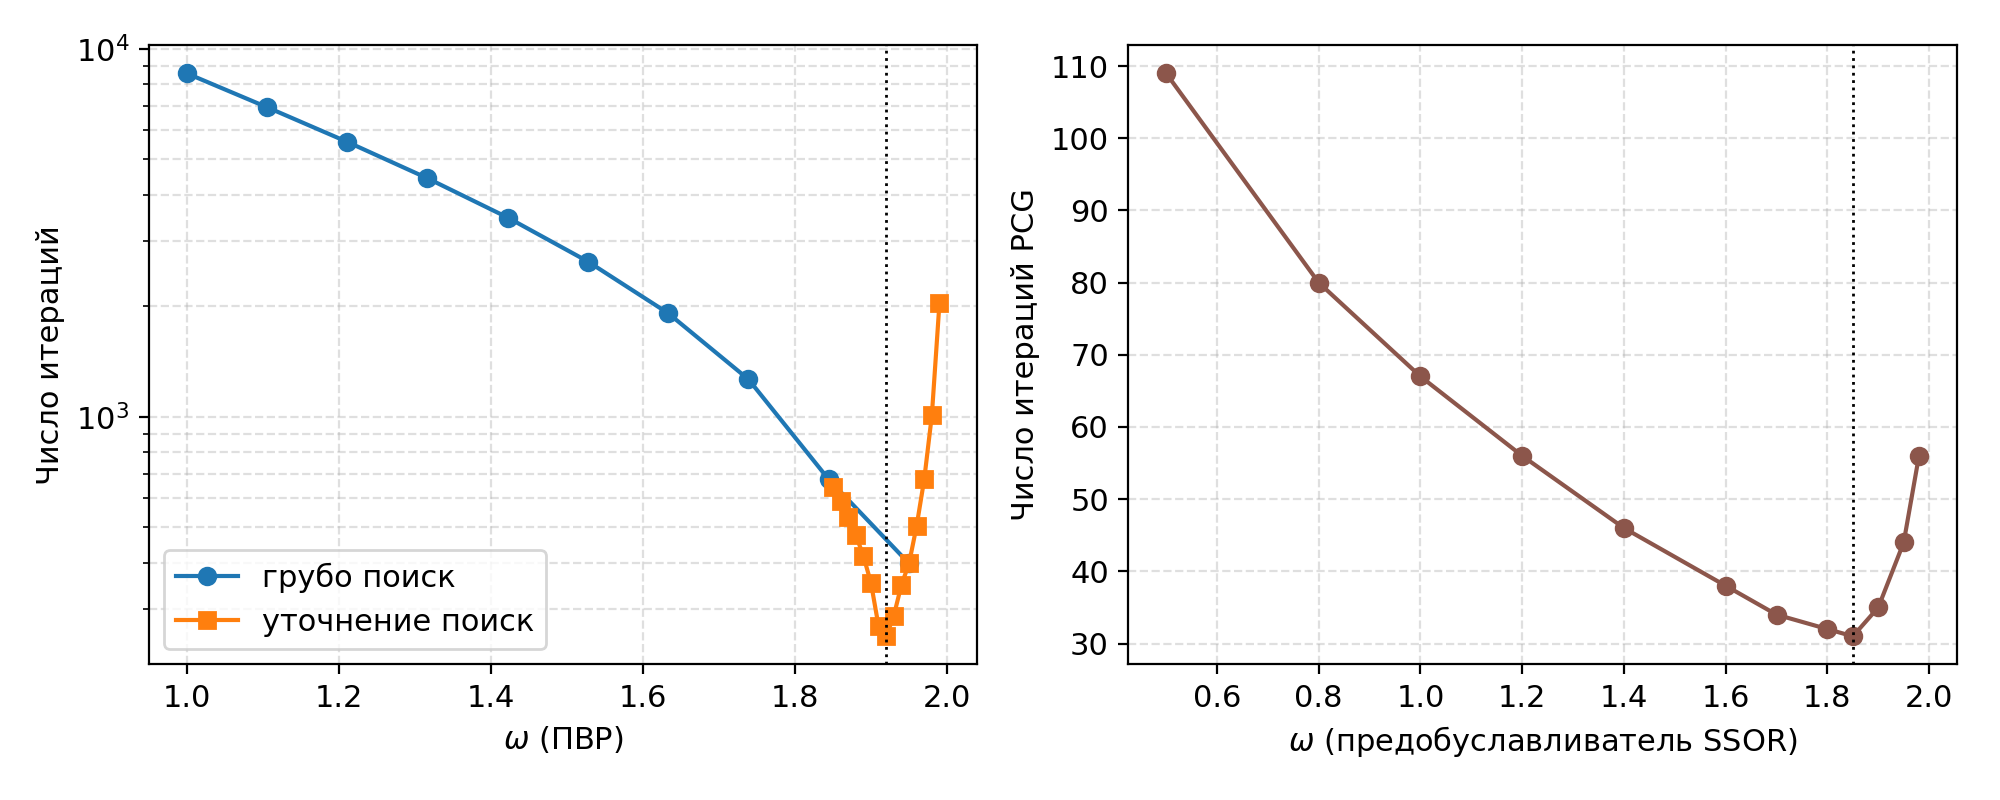
\includegraphics[width=15.5cm]{fig_omega_scan.png}
    \caption{Подбор параметров $\omega$ на сетке $N=64$: слева~--- ПВР-итерация, справа~--- предобуславливатель SSOR в PCG}
    \label{fig:omega}
\end{figure}

\textbf{Решение задачи варианта.} Результаты для $N=32$ и $N=64$ приведены в таблице~\ref{tab:stat}, кривые $\eta_s$~--- на рис.~\ref{fig:stat}. Для обоих размеров использован $\omega=1{,}92$, найденный на $N=64$; значение времени получено единственным запуском (интерпретатор Python, циклы по строкам), поэтому пригодно лишь для сравнения методов друг с другом.\par

\begin{table}[H]
\centering
\caption{Стационарные методы на задаче варианта E4 ($x^{(0)}=0$, максимум 10\,000 итераций)}
\label{tab:stat}
\small
\begin{tabular}{|c|l|c|c|c|c|c|}
\hline
$N$ & Метод & Итераций & Статус & $\eta_s$ & $\varepsilon_{res}$ & Время, с \\
\hline
32 & Якоби & 4\,144 & порог достигнут & $9{,}96\cdot10^{-9}$ & $1\cdot10^{-8}$ & 1,72 \\
32 & Зейдель & 2\,073 & порог достигнут & $9{,}95\cdot10^{-9}$ & $1\cdot10^{-8}$ & 0,922 \\
32 & ПВР ($\omega$=1,920) & 248 & порог достигнут & $7{,}42\cdot10^{-9}$ & $1\cdot10^{-8}$ & 0,129 \\
64 & Якоби & 10\,000 & \textbf{порог не достигнут} & $2{,}22\cdot10^{-5}$ & $1\cdot10^{-8}$ & 20,6 \\
64 & Зейдель & 8\,577 & порог достигнут & $9{,}99\cdot10^{-9}$ & $1\cdot10^{-8}$ & 17,9 \\
64 & ПВР ($\omega$=1,920) & 253 & порог достигнут & $7{,}85\cdot10^{-9}$ & $1\cdot10^{-8}$ & 0,579 \\
\hline
\end{tabular}
\end{table}

\begin{figure}[H]
    \centering
    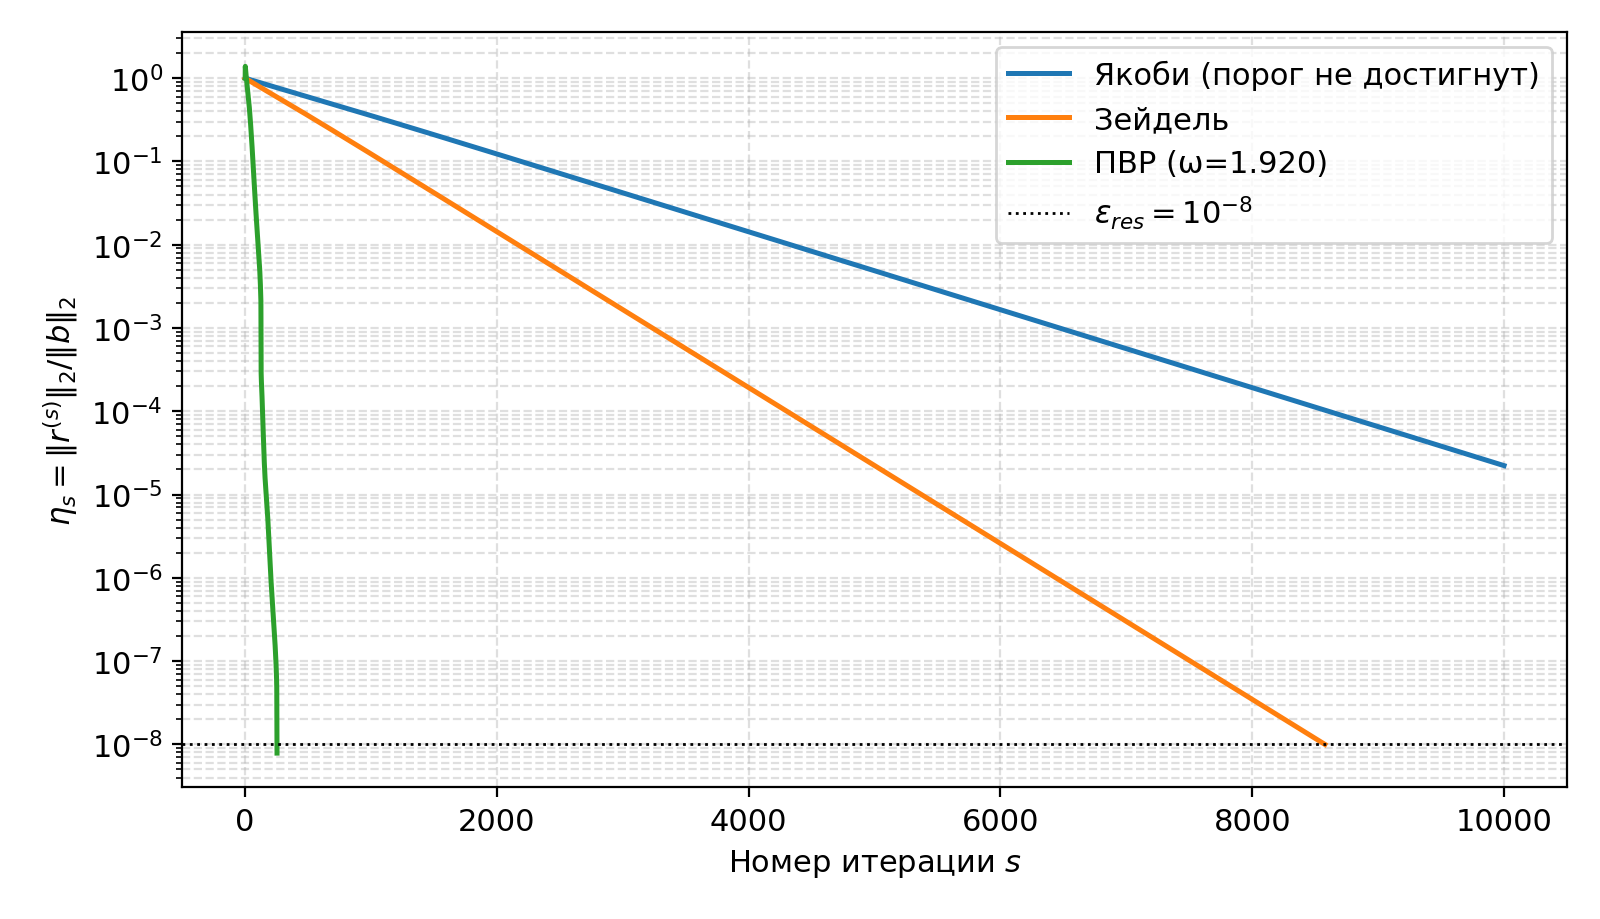
\includegraphics[width=14.5cm]{fig_conv_stationary_N64.png}
    \caption{Сходимость стационарных методов, $N=64$}
    \label{fig:stat}
\end{figure}

\textbf{Анализ.} (1) Метод Якоби на $N=64$ \textbf{не достиг порога} за 10\,000 итераций: $\eta=$ $2{,}22\cdot10^{-5}$. Это не стагнация: невязка убывает монотонно с постоянным темпом, на последних 1\,000 итерациях $\eta_{s+1}/\eta_s\approx0{,}99892$, что совпадает с $\rho(R_J)$ (таблица~\ref{tab:spec}). При таком темпе до порога оставалось бы ещё около 7\,152 итераций (всего порядка 17\,152), в согласии со спектральной оценкой $k_J^\text{оц}=17\,095$. (2) Метод Зейделя требует вдвое меньше итераций, чем Якоби ($N=32$: отношение 2,00), так как $\rho(R_{GS})=\rho(R_J)^2$; оценки $k^\text{оц}$ совпадают с фактическими числами итераций с точностью лучше 1\,\%, что одновременно подтверждает правильность реализации. (3) Число итераций Якоби и Зейделя растёт пропорционально $1/h^2\sim\mu(A)$ (таблица~\ref{tab:spec}). (4) ПВР с подобранным $\omega$ на $N=64$ требует в 34 раза меньше итераций, чем Зейдель, и примерно во столько же раз быстрее по времени (0,579 с против 17,9 с). Первые итерации ПВР немонотонны: максимум $\eta_s$ достигает 1{,}38 (рис.~\ref{fig:stat}), что характерно для сильной релаксации и не противоречит сходимости. (5) При $N=32$ параметр $\omega=1{,}92$, подобранный на $N=64$, выше оптимального для этой сетки ($\omega_{opt}^\text{теор}=1{,}828$), поэтому число итераций ПВР при $N=32$ нельзя считать минимально возможным.

\begin{table}[H]
\centering
\caption{Спектральные оценки и число итераций стационарных методов ($\varepsilon_{res}=10^{-8}$). Звёздочка: порог не достигнут за 10\,000 итераций; «---»: расчёт не проводился}
\label{tab:spec}
\footnotesize
\begin{tabular}{|c|c|c|c|c|c|c|c|}
\hline
$N$ & $\mu(A)$ & $\rho(R_J)$ & $k_J^{\text{оц}}$ & $k_J$ & $k_{GS}^{\text{оц}}$ & $k_{GS}$ & $\omega_{opt}^{\text{теор}}$ \\
\hline
32 & 888 & 0{,}99555 & 4\,130 & 4144 & 2\,065 & 2073 & 1{,}828 \\
64 & 3\,838 & 0{,}99892 & 17\,095 & 10000$^*$ & 8\,547 & 8577 & 1{,}911 \\
128 & 15\,948 & 0{,}99974 & 69\,507 & --- & 34\,753 & --- & 1{,}955 \\
\hline
\end{tabular}
\end{table}

\subsection{Этап 3. Методы сопряжённых градиентов}

\textbf{Выбор $\omega$ для SSOR.} Параметр $\omega$ предобуславливателя выполняет иную функцию, чем $\omega$ в ПВР: он не задаёт итерацию, а определяет оператор $P_\text{SSOR}$ и тем самым спектр $P^{-1}A$. При любом $\omega\in(0;2)$ предобуславливатель симметричен и положительно определён, а стоимость его применения от $\omega$ не зависит, поэтому $\omega$ выбирается по числу итераций PCG на $N=64$ (таблица~\ref{tab:ssorscan}, рис.~\ref{fig:omega}, справа). Минимум достигается внутри просмотренного интервала при $\omega=1{,}85$ (31 итераций); соседние значения $1{,}8$ и $1{,}9$ дают 32 и 35 итераций, т.\,е. минимум пологий. Найденное значение является наилучшим среди проверенных; оно использовано на всех сетках и при проверке на тестовой системе.\par

\begin{table}[H]
\centering
\caption{Подбор параметра $\omega$ предобуславливателя SSOR (PCG, $N=64$)}
\label{tab:ssorscan}
\small
\begin{tabular}{|c|c|c|c|}
\hline
$\omega$ & Итераций & $\omega$ & Итераций \\
\hline
$0{,}50$ & $109$ & $1{,}70$ & $34$ \\
$0{,}80$ & $80$ & $1{,}80$ & $32$ \\
$1{,}00$ & $67$ & $1{,}85$ & $31$ \\
$1{,}20$ & $56$ & $1{,}90$ & $35$ \\
$1{,}40$ & $46$ & $1{,}95$ & $44$ \\
$1{,}60$ & $38$ & $1{,}98$ & $56$ \\
\hline
\end{tabular}
\end{table}

\textbf{Проверка на системе с известным решением} (та же $b^*=Au^*$, $N=32$). Результаты в таблице~\ref{tab:test_cg}. Во всех случаях пересчитанная невязка не превышает $10^{-8}$, а $\delta_s/\eta_s$ лежит в пределах от 0,29 до 0,49, то есть для методов Крылова погрешность решения СЛАУ того же порядка, что невязка, и оценка $\delta_s\le\mu(A)\eta_s$ выполняется с запасом более двух порядков.\par

\begin{table}[H]
\centering
\caption{Тестовая система ($N=32$, порог $\varepsilon_{res}=10^{-8}$): невязка и погрешность методов CG/PCG}
\label{tab:test_cg}
\small
\begin{tabular}{|l|c|c|c|c|c|}
\hline
Метод & Итераций & $\eta_s$ & $\delta_s$ & $\delta_s/\eta_s$ & $\mu(A)\,\eta_s$ \\
\hline
CG & 145 & $7{,}97\cdot10^{-9}$ & $3{,}84\cdot10^{-9}$ & 0,48 & $7{,}08\cdot10^{-6}$ \\
PCG (диаг.) & 106 & $8{,}71\cdot10^{-9}$ & $4{,}28\cdot10^{-9}$ & 0,49 & $7{,}73\cdot10^{-6}$ \\
PCG (SSOR, $\omega$=1,85) & 26 & $4{,}81\cdot10^{-9}$ & $1{,}38\cdot10^{-9}$ & 0,29 & $4{,}27\cdot10^{-6}$ \\
\hline
\end{tabular}
\end{table}

\textbf{Основные расчёты.} Результаты для $N=32,\,64,\,128$ ($x^{(0)}=0$, $\varepsilon_{res}=10^{-8}$) даны в таблицах~\ref{tab:krylov} и~\ref{tab:cost}. Время измерено как медиана трёх запусков после одного пробного; $t_\text{подг}$~--- время построения предобуславливателя (для SSOR~--- матрицы $B$ и $B^T$), $t_\text{итер}$~--- время итераций, $t_\Sigma=t_\text{подг}+t_\text{итер}$. Объём памяти CSR-матрицы указан в байтах; плотная матрица при $N=128$ заняла бы 2,02~ГБ (в 1\,996 раз больше, чем CSR: 1\,010\,020~Б).\par

\begin{table}[H]
\centering
\caption{Результаты методов CG и PCG ($x^{(0)}=0$)}
\label{tab:krylov}
\small
\begin{tabular}{|c|l|c|c|c|c|c|}
\hline
$N$ & Метод & Итераций & Матвекс & $\eta_s$ & $\varepsilon_{res}$ & Порог \\
\hline
32 & CG & 109 & 112 & $8{,}00\cdot10^{-9}$ & $1\cdot10^{-8}$ & да \\
32 & PCG (диаг.) & 79 & 81 & $8{,}01\cdot10^{-9}$ & $1\cdot10^{-8}$ & да \\
32 & PCG (SSOR, $\omega=1{,}85$) & 26 & 27 & $8{,}75\cdot10^{-9}$ & $1\cdot10^{-8}$ & да \\
64 & CG & 242 & 247 & $8{,}54\cdot10^{-9}$ & $1\cdot10^{-8}$ & да \\
64 & PCG (диаг.) & 162 & 166 & $9{,}36\cdot10^{-9}$ & $1\cdot10^{-8}$ & да \\
64 & PCG (SSOR, $\omega=1{,}85$) & 31 & 32 & $5{,}96\cdot10^{-9}$ & $1\cdot10^{-8}$ & да \\
128 & CG & 522 & 533 & $9{,}04\cdot10^{-9}$ & $1\cdot10^{-8}$ & да \\
128 & PCG (диаг.) & 331 & 338 & $9{,}07\cdot10^{-9}$ & $1\cdot10^{-8}$ & да \\
128 & PCG (SSOR, $\omega=1{,}85$) & 47 & 48 & $8{,}78\cdot10^{-9}$ & $1\cdot10^{-8}$ & да \\
\hline
\end{tabular}
\end{table}

\begin{table}[H]
\centering
\caption{Стоимость расчётов CG/PCG (медиана трёх замеров после пробного запуска)}
\label{tab:cost}
\footnotesize
\begin{tabular}{|c|l|c|c|c|c|c|c|c|}
\hline
$N$ & Метод & $n$ & $\mathrm{nnz}$ & CSR, Б & $t_{\text{подг}}$, с & $t_{\text{итер}}$, с & $t_{\Sigma}$, с & мс/итер. \\
\hline
32 & CG & 900 & 4\,380 & 56\,164 & 0,0000 & 0,0016 & 0,0016 & 0,015 \\
32 & PCG (диаг.) & 900 & 4\,380 & 56\,164 & 0,0000 & 0,0014 & 0,0014 & 0,018 \\
32 & PCG (SSOR) & 900 & 4\,380 & 56\,164 & 0,0005 & 0,021 & 0,021 & 0,807 \\
64 & CG & 3\,844 & 18\,972 & 243\,044 & 0,0000 & 0,0077 & 0,0077 & 0,032 \\
64 & PCG (диаг.) & 3\,844 & 18\,972 & 243\,044 & 0,0000 & 0,0064 & 0,0064 & 0,039 \\
64 & PCG (SSOR) & 3\,844 & 18\,972 & 243\,044 & 0,0007 & 0,043 & 0,044 & 1,401 \\
128 & CG & 15\,876 & 78\,876 & 1\,010\,020 & 0,0000 & 0,058 & 0,058 & 0,112 \\
128 & PCG (диаг.) & 15\,876 & 78\,876 & 1\,010\,020 & 0,0001 & 0,044 & 0,044 & 0,133 \\
128 & PCG (SSOR) & 15\,876 & 78\,876 & 1\,010\,020 & 0,0018 & 0,175 & 0,177 & 3,731 \\
\hline
\end{tabular}
\end{table}

\begin{figure}[H]
    \centering
    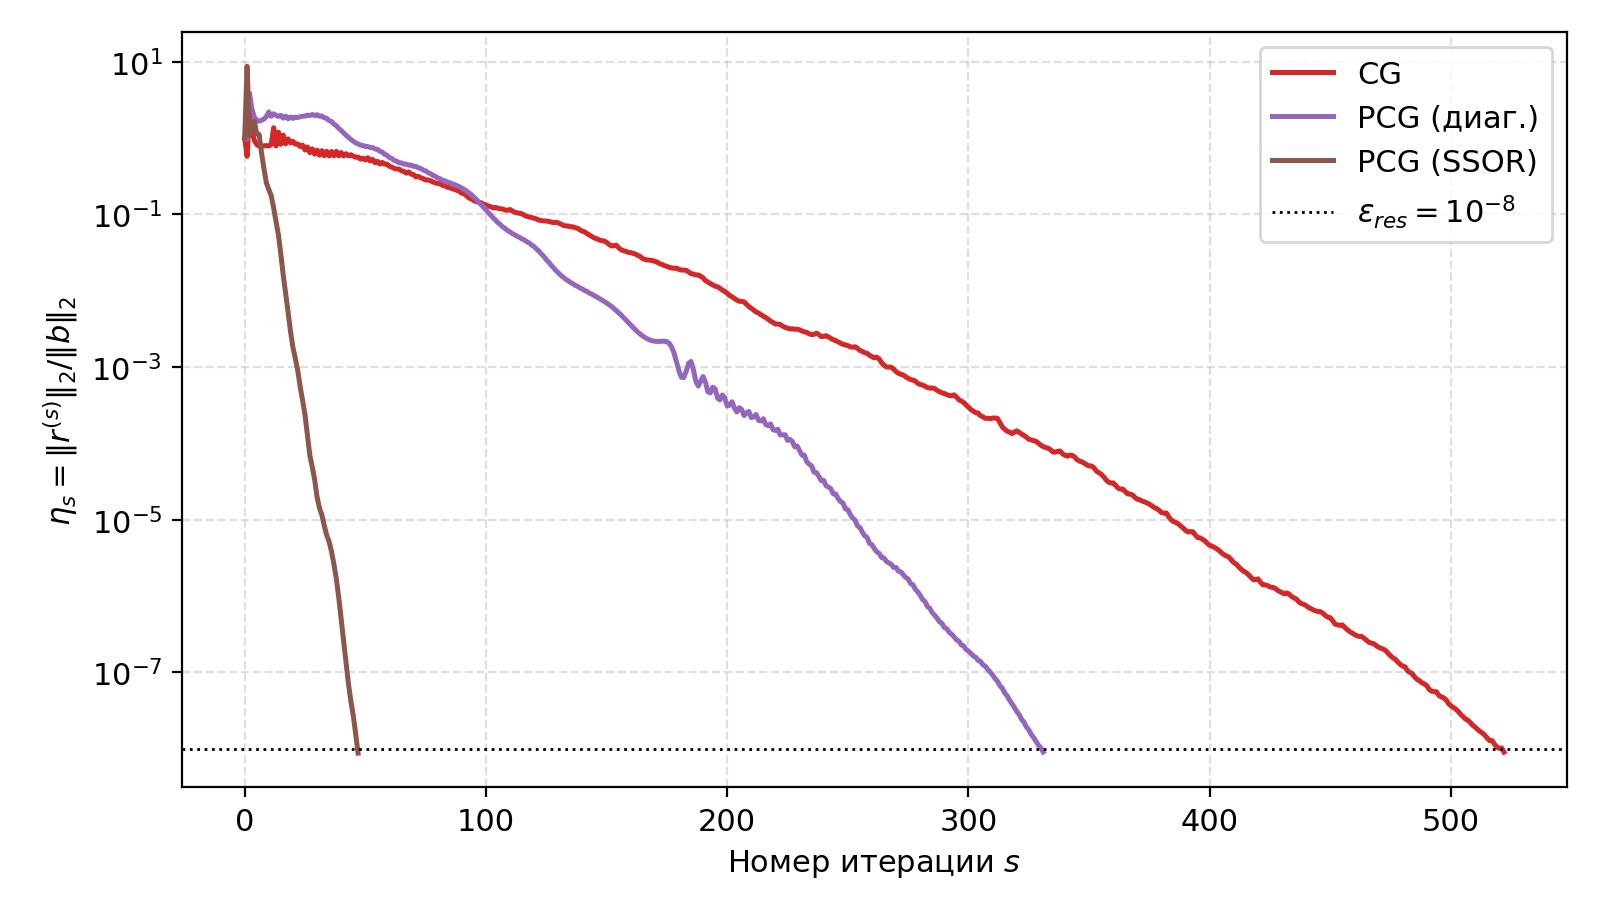
\includegraphics[width=14.5cm]{fig_conv_krylov_N128.png}
    \caption{Сходимость CG и PCG, $N=128$ (пунктирная линия~--- порог $\varepsilon_{res}$)}
    \label{fig:krylov}
\end{figure}

\begin{figure}[H]
    \centering
    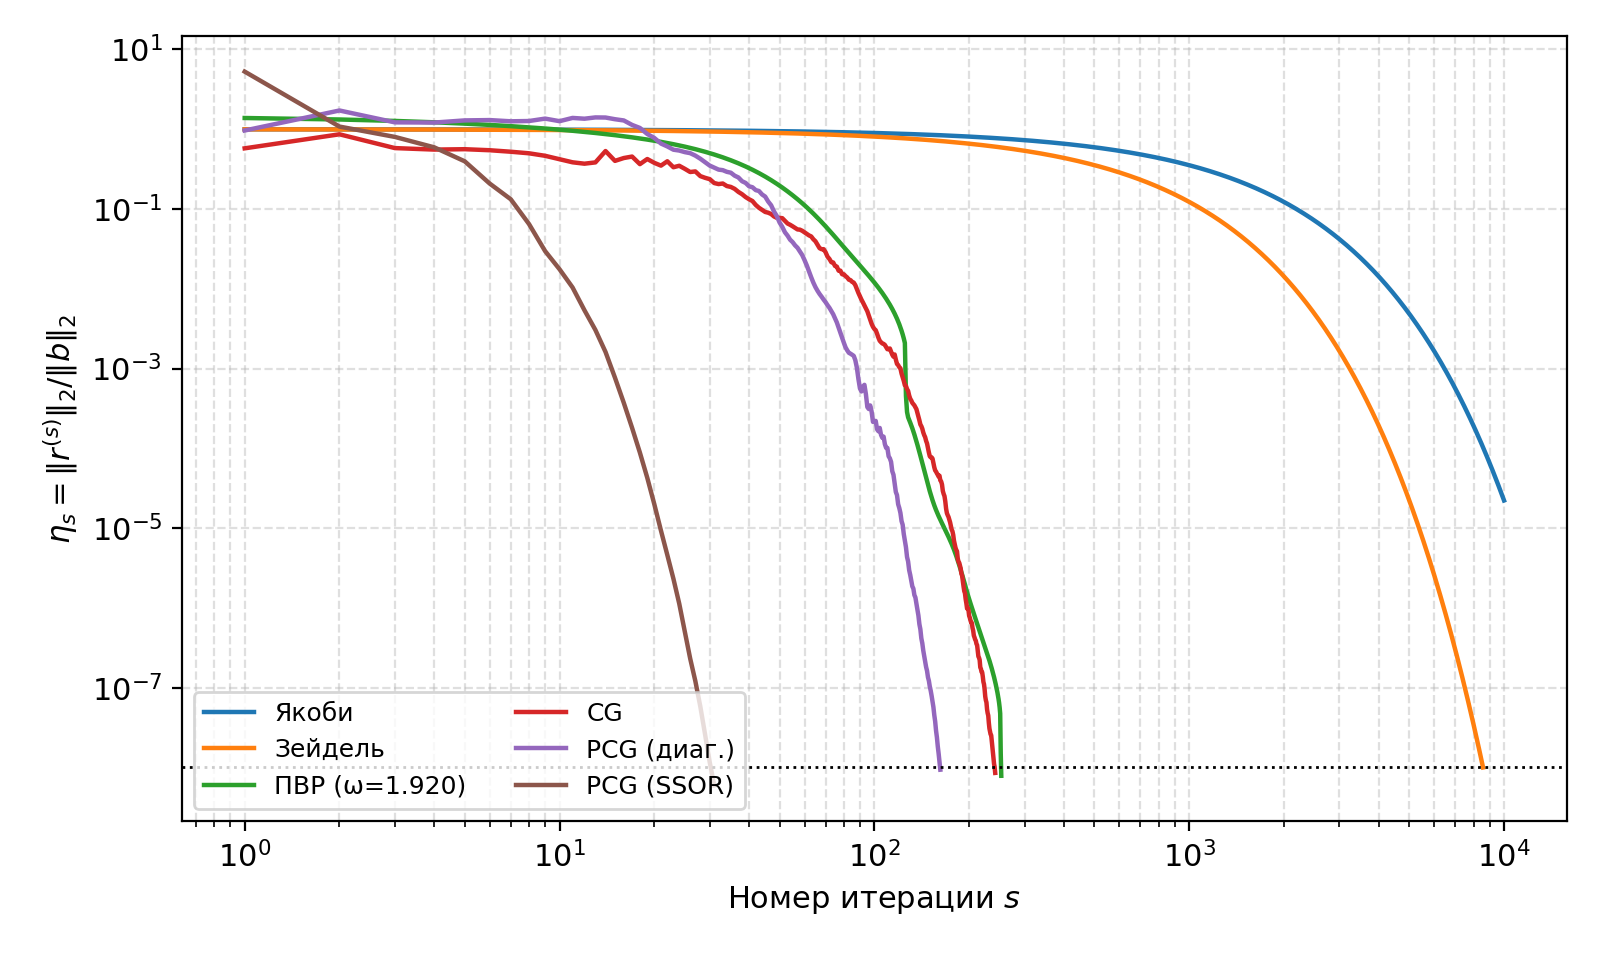
\includegraphics[width=14.5cm]{fig_conv_all_N64.png}
    \caption{Сходимость всех шести методов на сетке $N=64$ (логарифмические шкалы по обеим осям)}
    \label{fig:all}
\end{figure}

\begin{figure}[H]
    \centering
    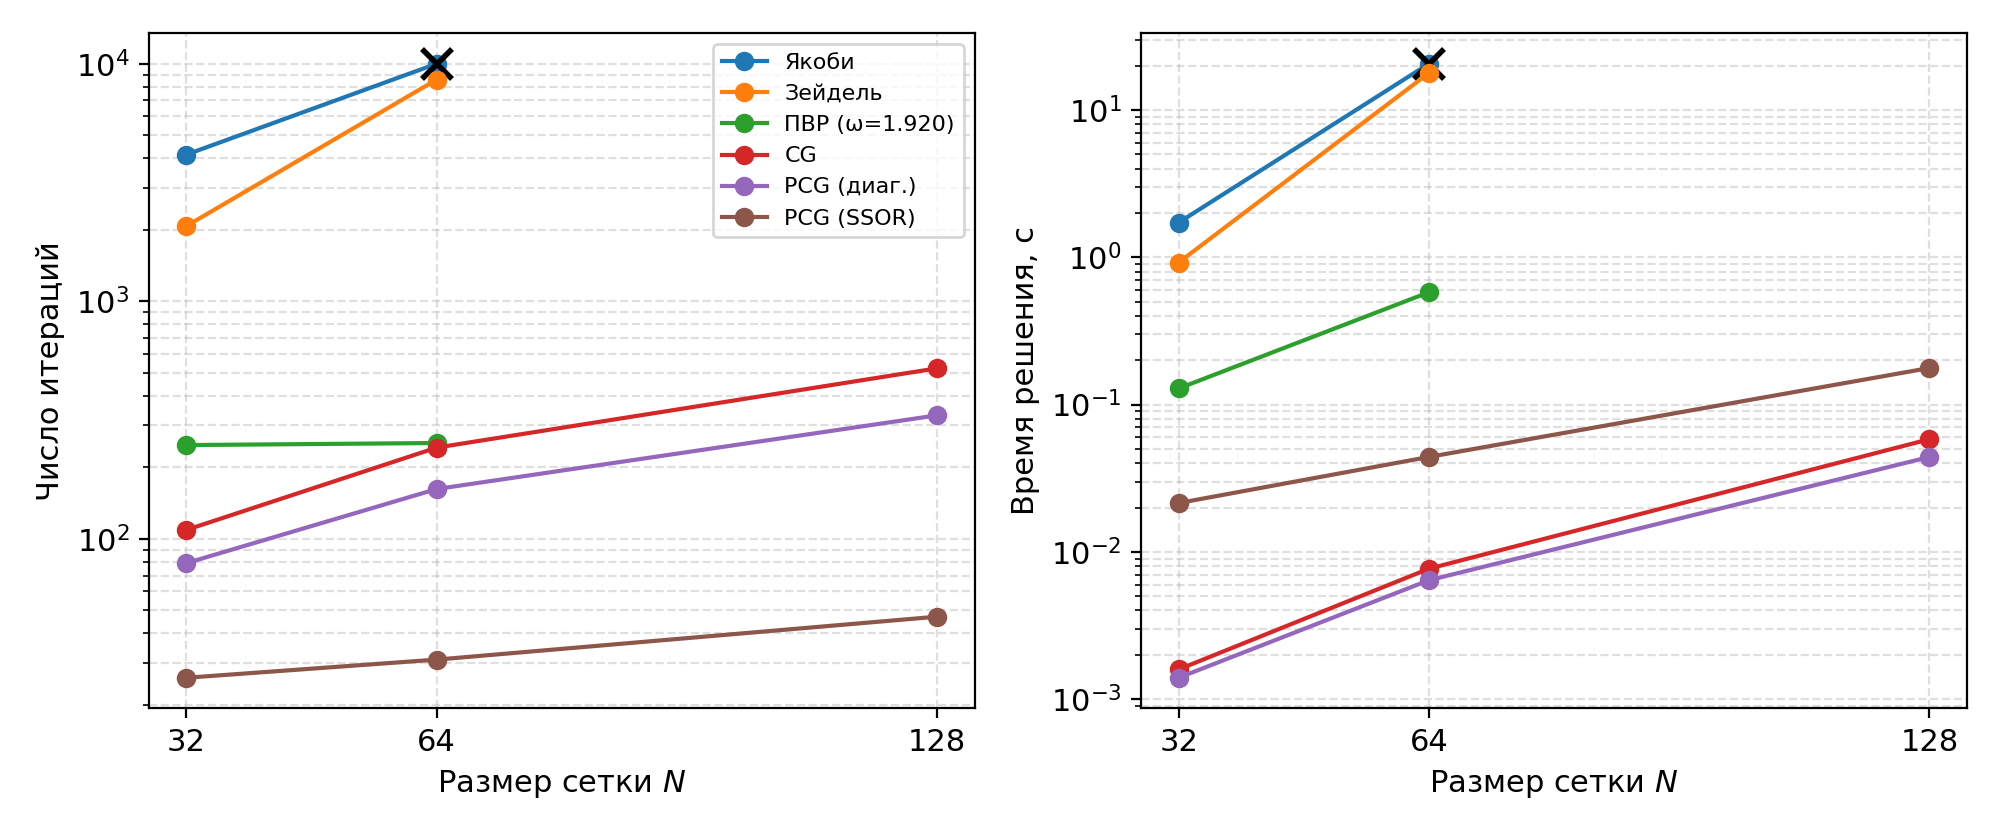
\includegraphics[width=16cm]{fig_iters_time_vs_N.png}
    \caption{Число итераций и время решения в зависимости от $N$ (крестик~--- порог не достигнут; для ПВР при $N=128$ расчёт не проводился)}
    \label{fig:iters}
\end{figure}

\textbf{Анализ.}\par

\textit{Размер матрицы и обусловленность.} Число обусловленности растёт как $N^2$ (отношения $\mu(A)$ при удвоении $N$: 4,32 и 4,15), а число итераций CG~--- как $N\sim\sqrt{\mu(A)}$: отношения числа итераций при удвоении $N$ равны 2,22 и 2,16. Оценка $\frac12\sqrt\kappa\ln(2/\varepsilon)$ (таблица~\ref{tab:cond}) даёт верхнюю границу: для CG и диагонального предобуславливателя фактическое число итераций примерно в 2,5 раза меньше оценки, для SSOR"--- в 1,2--1,9 раза.\par

\textit{Диагональный предобуславливатель.} Коэффициент $a$ меняется всего в 3 раза, поэтому диагональ $A$ почти постоянна и масштабирование мало меняет спектр: $\kappa(D^{-1}A)\approx\mu(A)/2$, число итераций уменьшается лишь в 1,58 раза (при $N=128$), а закон роста сохраняется (отношения 2,05 и 2,04).\par

\textit{SSOR.} Предобуславливатель SSOR уменьшает эффективное $\kappa$ с $\sim10^4$ до $\sim10^2$ (таблица~\ref{tab:cond}: $\kappa(P^{-1}A)\approx 10,1;\ 23,8;\ 81,3$ при $N=32;\,64;\,128$), так что число итераций падает в 11,1 раза при $N=128$ и растёт заметно медленнее ($\kappa\sim N$, число итераций $\sim\sqrt N$; отношения 1,19 и 1,52). Оценка $\kappa(P^{-1}A)$ по числам Ритца приближённая (наименьшее число Ритца сходится сверху).\par

\begin{table}[H]
\centering
\caption{Эффективная обусловленность и оценка числа итераций CG/PCG: $s_{\text{оц}}=\frac12\sqrt{\kappa}\ln(2/\varepsilon)$ при $\varepsilon=10^{-8}$ (оценка сверху для энергетической нормы)}
\label{tab:cond}
\scriptsize
\begin{tabular}{|c|c|c|c|c|c|c|c|c|c|}
\hline
$N$ & \multicolumn{3}{c|}{CG: $\mu(A)$, $s_{\text{оц}}$, факт} & \multicolumn{3}{c|}{диаг.: $\kappa(D^{-1}A)$, $s_{\text{оц}}$, факт} & \multicolumn{3}{c|}{SSOR: $\kappa(P^{-1}A)$, $s_{\text{оц}}$, факт} \\
\hline
32 & 888 & 285 & 109 & 448 & 203 & 79 & 10,1 & 31 & 26 \\
64 & 3\,838 & 593 & 242 & 1\,856 & 412 & 162 & 23,8 & 47 & 31 \\
128 & 15\,948 & 1207 & 522 & 7\,547 & 831 & 331 & 81,3 & 87 & 47 \\
\hline
\end{tabular}
\end{table}

\textit{Число итераций и время.} Малое число итераций не гарантирует малого времени. На сетке $N=128$ PCG с SSOR выполняет в 11,1 раза меньше итераций, чем CG, но по общему времени медленнее ($t_\Sigma=0,177$~с против 0,058~с для CG, в 3,0 раза). Причина видна из замеров стоимости элементарных операций при $N=128$: умножение $Ap$ занимает 58~мкс, применение диагонального $P^{-1}$~--- 12~мкс, а применение $P_\text{SSOR}^{-1}$ (два вызова \texttt{spsolve\_triangular})~--- 3,80~мс, то есть около 66 матвеков. Таким образом, выигрыш по итерациям поглощается стоимостью универсальной треугольной подстановки; для получения выигрыша по времени её нужно заменять оптимизированной (компилируемой) реализацией. Диагональный предобуславливатель почти ничего не стоит и даёт небольшой, но реальный выигрыш по времени ($0,044$~с против 0,058~с при $N=128$). Памяти PCG требует столько же, сколько CG, плюс $O(n)$ для диагонали либо $O(\mathrm{nnz})$ для $B$, $B^T$.\par

\subsection{Этап 4. Независимая проверка решения}

Контрольные решения получены прямым решателем \texttt{spsolve} и библиотечным CG (\texttt{rtol}=$10^{-10}$, \texttt{atol}=0); код возврата и невязка пересчитаны независимо (таблица~\ref{tab:ctrl}). Решения собственных методов сравнены с контрольными в относительных нормах $L_2$ и $L_\infty$ (таблица~\ref{tab:cmp}).\par

\begin{table}[H]
\centering
\caption{Контрольные решения и независимо пересчитанные невязки}
\label{tab:ctrl}
\small
\begin{tabular}{|c|l|c|c|c|}
\hline
$N$ & Решатель & Код возврата & $\eta$ & $t$, с \\
\hline
32 & spsolve & --- & $3{,}47\cdot10^{-14}$ & 0,0023 \\ \hline
32 & scipy.sparse.linalg.cg, rtol=$10^{-10}$ & 0 & $6{,}99\cdot10^{-11}$ & ---  \\
64 & spsolve & --- & $1{,}43\cdot10^{-13}$ & 0,012 \\ \hline
64 & scipy.sparse.linalg.cg, rtol=$10^{-10}$ & 0 & $9{,}62\cdot10^{-11}$ & ---  \\
128 & spsolve & --- & $6{,}03\cdot10^{-13}$ & 0,061 \\ \hline
128 & scipy.sparse.linalg.cg, rtol=$10^{-10}$ & 0 & $9{,}77\cdot10^{-11}$ & ---  \\
\hline
\end{tabular}
\end{table}

\begin{table}[H]
\centering
\caption{Относительное расхождение собственных решений с контрольными}
\label{tab:cmp}
\small
\begin{tabular}{|c|l|c|c|c|c|}
\hline
$N$ & Метод & $L_2$ (spsolve) & $L_\infty$ (spsolve) & $L_2$ (SciPy CG) & $L_\infty$ (SciPy CG) \\
\hline
32 & CG & $1{,}56\cdot10^{-10}$ & $2{,}35\cdot10^{-10}$ & $1{,}55\cdot10^{-10}$ & $2{,}35\cdot10^{-10}$ \\
32 & PCG (диаг.) & $2{,}08\cdot10^{-10}$ & $3{,}18\cdot10^{-10}$ & $2{,}08\cdot10^{-10}$ & $3{,}18\cdot10^{-10}$ \\
32 & PCG (SSOR) & $1{,}56\cdot10^{-10}$ & $3{,}60\cdot10^{-10}$ & $1{,}56\cdot10^{-10}$ & $3{,}59\cdot10^{-10}$ \\
64 & CG & $1{,}06\cdot10^{-10}$ & $1{,}90\cdot10^{-10}$ & $1{,}06\cdot10^{-10}$ & $1{,}91\cdot10^{-10}$ \\
64 & PCG (диаг.) & $1{,}56\cdot10^{-10}$ & $2{,}29\cdot10^{-10}$ & $1{,}56\cdot10^{-10}$ & $2{,}28\cdot10^{-10}$ \\
64 & PCG (SSOR) & $2{,}57\cdot10^{-10}$ & $3{,}04\cdot10^{-10}$ & $2{,}57\cdot10^{-10}$ & $3{,}02\cdot10^{-10}$ \\
128 & CG & $7{,}49\cdot10^{-11}$ & $1{,}13\cdot10^{-10}$ & $7{,}48\cdot10^{-11}$ & $1{,}12\cdot10^{-10}$ \\
128 & PCG (диаг.) & $1{,}22\cdot10^{-10}$ & $2{,}14\cdot10^{-10}$ & $1{,}23\cdot10^{-10}$ & $2{,}14\cdot10^{-10}$ \\
128 & PCG (SSOR) & $1{,}44\cdot10^{-10}$ & $2{,}44\cdot10^{-10}$ & $1{,}44\cdot10^{-10}$ & $2{,}44\cdot10^{-10}$ \\
\hline
\end{tabular}
\end{table}

Библиотечный CG завершился с кодом 0 для всех сеток, расхождение двух контрольных решений не превышает $2{,}75\cdot10^{-12}$. Собственные решения отличаются от контрольных на $7{,}48\cdot10^{-11}$--$3{,}60\cdot10^{-10}$, то есть на два порядка меньше, чем $\varepsilon_{res}=10^{-8}$: невязка на пороге оценивает ошибку сверху, а реальная ошибка гладкого решения существенно меньше. Согласие трёх независимых решателей подтверждает, что собственные реализации решают одну и ту же СЛАУ верно, но не доказывает точность схемы, по которой матрица получена из краевой задачи.

\subsection{Этап 5. Результаты, поле решения и физическая интерпретация}

Сводные результаты приведены в таблицах~\ref{tab:stat}, \ref{tab:krylov}, \ref{tab:cost} и в CSV-файле; графики сходимости~--- рис.~\ref{fig:stat}--\ref{fig:all}, зависимость числа итераций от $N$~--- рис.~\ref{fig:iters}. Поле потенциала и модуль напряжённости на сетке $N=128$ (решение PCG, совпадающее с контрольным) показаны на рис.~\ref{fig:field}.\par

\begin{figure}[H]
    \centering
    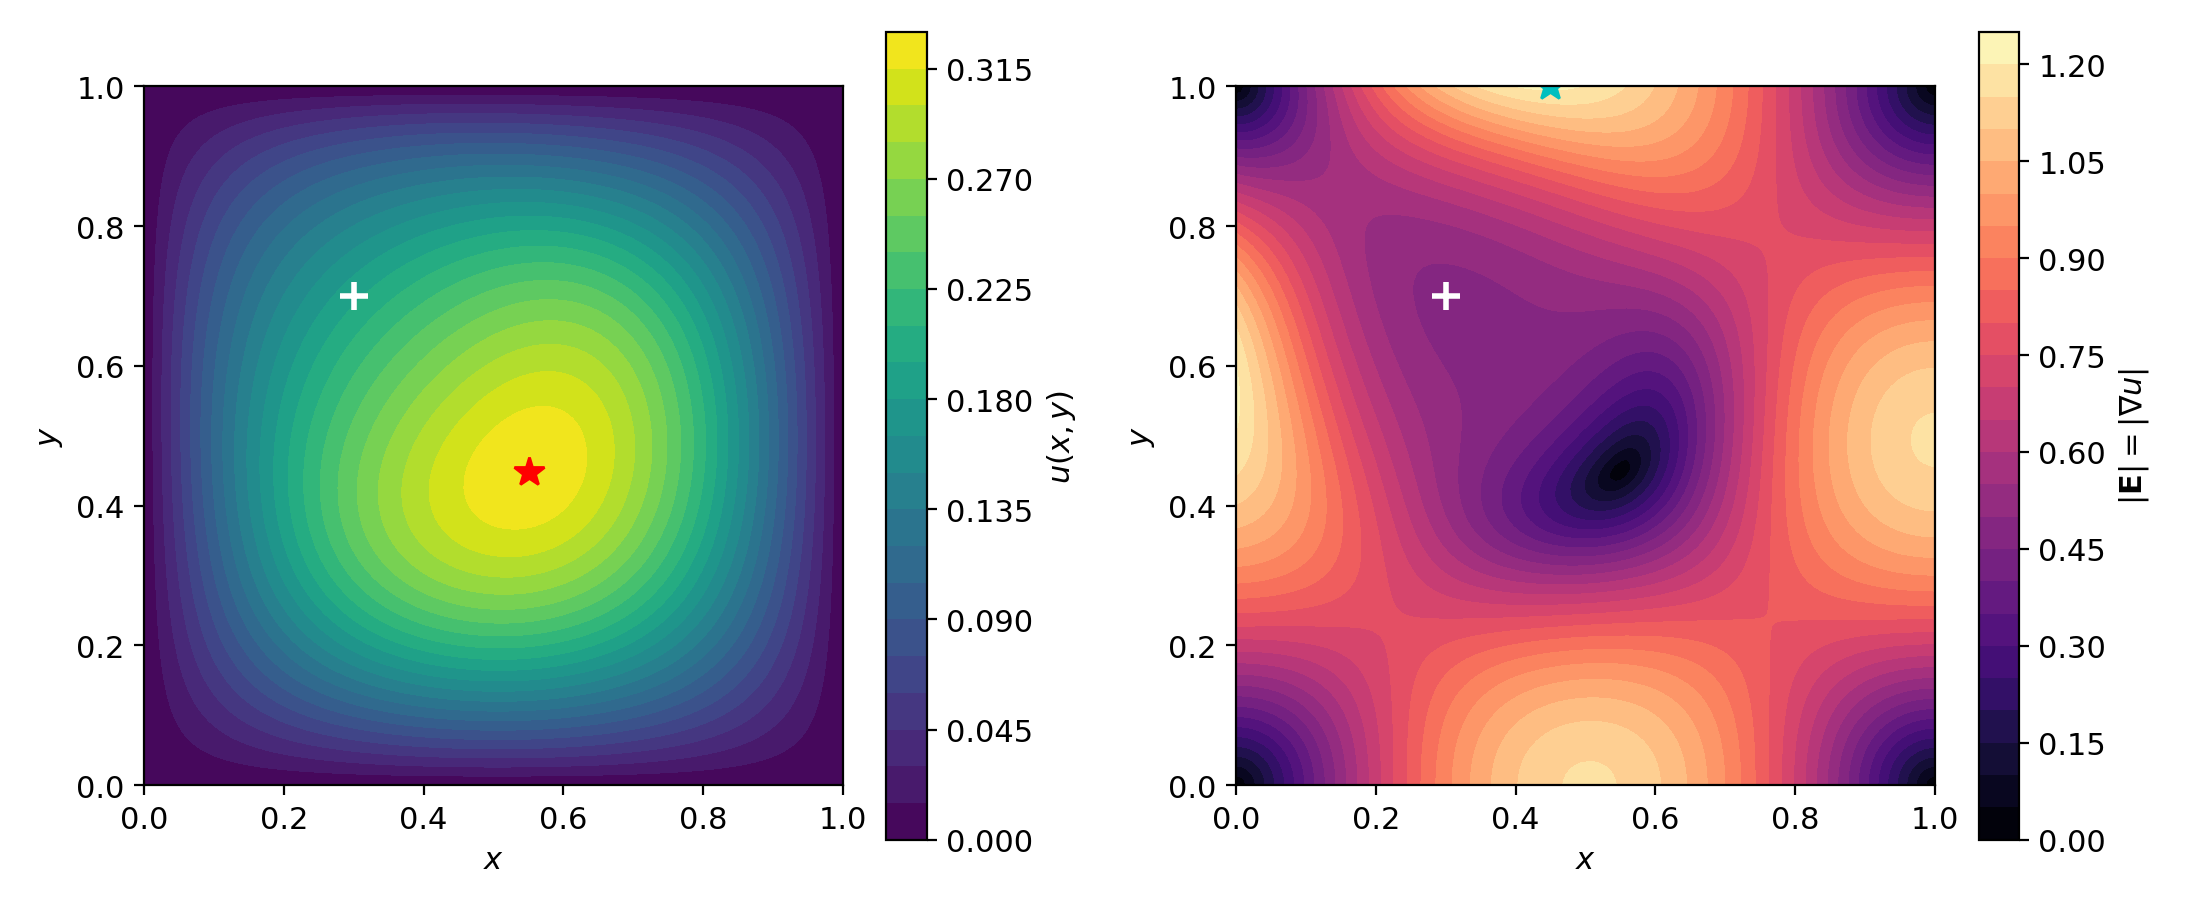
\includegraphics[width=16.5cm]{fig_field_N128.png}
    \caption{Потенциал $u(x,y)$ (слева) и модуль напряжённости $|\mathbf E|=|\nabla u|$ (справа), $N=128$; звезда~--- максимум, крестик~--- центр включения $a(x,y)$ в точке $(0{,}3;\,0{,}7)$}
    \label{fig:field}
\end{figure}

\begin{table}[H]
\centering
\caption{Физические характеристики решения ($N=128$, безразмерные величины)}
\label{tab:phys}
\small
\begin{tabular}{|l|c|}
\hline
Характеристика & Значение \\
\hline
Максимум потенциала $u_{\max}$ & $0{,}3273$ в точке $(0{,}551;\;0{,}449)$ \\
Максимум $|\mathbf E|=|\nabla u|$ на замкнутой сетке & $1{,}2125$ в точке $(0{,}449;\;1{,}000)$ \\
Максимум $|\mathbf E|$ среди внутренних узлов & $1{,}1931$ в точке $(0{,}457;\;0{,}992)$ \\
$|\mathbf E|$ в центре области $(0{,}5;\,0{,}5)$ & $0{,}2744$ \\
Поток $\mathbf D=a\mathbf E$ через левую / правую сторону & $1{,}3222$ / $1{,}1093$ \\
Поток $\mathbf D$ через нижнюю / верхнюю сторону & $1{,}1093$ / $1{,}3222$ \\
Суммарный поток через границу $\Phi$ & $4{,}86292$ \\
Полный заряд $Q=h^2\sum f_{ij}$ (численный) / $48/\pi^2$ (точный) & $4{,}86292$ / $4{,}86342$ \\
$u_{\max}$ при $N=32\,/\,64\,/\,128$ & $0{,}3275\,/\,0{,}3272\,/\,0{,}3273$ \\
\hline
\end{tabular}
\end{table}

Напряжённость $\mathbf E=-\nabla u$ вычислена центральными разностями во внутренних узлах и односторонними разностями второго порядка на границе (значения даны в безразмерных единицах, масштаб $U_0/L$ при обезразмеривании не задан).\par

\textbf{Интерпретация.} (1) Потенциал имеет единственный максимум $u_{\max}=0{,}3273$ в точке $(0{,}551;\,0{,}449)$, а не в центре области $(0{,}5;\,0{,}5)$, где сосредоточен заряд: максимум смещён вдоль диагонали $x+y=1$ от области повышенной диэлектрической проницаемости, расположенной в точке $(0{,}3;\,0{,}7)$. Решение симметрично относительно этой диагонали, поскольку и $a$, и $f$ симметричны относительно отражения $(x,y)\mapsto(1-y,1-x)$; численно это проявляется в равенстве потоков через левую и верхнюю стороны ($1{,}322$) и через правую и нижнюю ($1{,}109$). (2) Поток вектора $\mathbf D=a\mathbf E$ через границу равен полному заряду (закон Гаусса): $\Phi=4{,}8629$ при точном $Q=48/\pi^2$ (отличие $0,010\,\%$ определяется аппроксимацией интеграла суммой). Через левую и верхнюю стороны, ближайшие к области повышенной проницаемости, уходит на 19\,\% больше потока, чем через правую и нижнюю. (3) Максимум напряжённости $|\mathbf E|_{\max}=1{,}212$ достигается \emph{на заземлённой границе}: на верхней стороне при $x=0{,}449$ (и симметрично на левой), а не внутри области; в центре $|\mathbf E|=0{,}274$, так как вблизи максимума потенциала поле мало. Максимум среди внутренних узлов равен 1{,}193 (он также приходится на ряд узлов, соседних с границей), то есть вычисление только по внутренним узлам занижает значение. (4) Значение $u_{\max}$ при $N=32,\,64,\,128$ меняется менее чем на 0,1\,\%, поэтому физический вывод устойчив по сетке (это не оценка погрешности дискретизации).\par

\textbf{Стагнация и недостижение порога.} Единственный случай недостижения порога~--- метод Якоби на $N=64$ ($2{,}22\cdot10^{-5}$ после 10\,000 итераций); стагнации (прекращения убывания невязки) нет ни в одном расчёте: до достижения порога $\eta_s$ убывает с постоянным темпом (стационарные методы) либо с небольшими немонотонными участками (CG/PCG). Ни на каком окне из 50 итераций невязка не перестала убывать: наибольшее отношение $\eta_{s+50}/\eta_s$ по всем расчётам равно 0{,}96. Рекуррентная невязка CG/PCG в момент остановки отличается от истинной, пересчитанной по найденному $x$, не более чем на $1{,}2\cdot10^{-6}$ (относительно), так что потери точности из-за округления не наблюдалось.\par

\section{Вывод}

\begin{enumerate}
  \item Матрица варианта E4 по формуле (3) собрана в формате CSR и проверена: не более пяти ненулевых элементов в строке, симметрия до уровня округления, положительная диагональ, $z^TAz>0$, разложение Холецкого без сдвига выполнимо, независимая векторизованная реализация формулы совпала с $Au$ до $10^{-16}$. Память CSR при $N=128$ составила 1\,010\,020~Б вместо 2,02~ГБ плотной матрицы.
  \item Скорость стационарных методов определяется $\rho(R_J)\to1$ при $h\to0$: число итераций Якоби и Зейделя растёт как $N^2$, метод Якоби на $N=64$ не достиг порога за 10\,000 итераций (требуется около 17\,152). Оценки по спектру ($k_J^\text{оц}$, $k_{GS}^\text{оц}$) совпали с фактическими числами итераций с точностью лучше 1\,\%. ПВР с $\omega=1{,}92$ (наилучшее среди проверенных; теоретически $\omega_{opt}=1{,}911$) сократил число итераций по сравнению с Зейделем в 34 раза.
  \item На тестовой системе с известным решением невязка и погрешность согласуются с $\delta_s\le\mu(A)\eta_s$; для методов Якоби и Зейделя $\delta_s\approx 13,6\,\eta_s$, для методов Крылова $\delta_s\sim\eta_s$. Малая невязка не определяет погрешность напрямую, поэтому для основной системы вывод о точности делается с учётом $\mu(A)$.
  \item Число итераций CG растёт как $N\sim\sqrt{\mu(A)}$ (отношения 2,22 и 2,16 при удвоении $N$). Диагональный предобуславливатель в этой задаче даёт лишь $\approx1,58$-кратное сокращение ($\kappa(D^{-1}A)\approx\mu(A)/2$), SSOR с $\omega=1{,}85$~--- сокращение в 11,1 раза при $N=128$ и более слабый рост числа итераций ($\kappa\sim N$).
  \item Число итераций не равно времени: в реализации через \texttt{spsolve\_triangular} применение $P_\text{SSOR}^{-1}$ стоит около 66 матвеков, и PCG с SSOR оказывается в 3,0 раза медленнее CG при $N=128$; самым быстрым по времени в данной реализации является PCG с диагональным предобуславливателем.
  \item Собственные решения CG/PCG совпали с решениями \texttt{spsolve} и библиотечного CG (код возврата 0) до $3{,}60\cdot10^{-10}$ в нормах $L_2$ и $L_\infty$ на всех сетках.
  \item Физический результат: потенциал максимален ($u_{\max}=0{,}3273$) в точке $(0{,}551;\,0{,}449)$, смещённой от области повышенной проницаемости; поток вектора $\mathbf D$ через границу равен полному заряду; максимум напряжённости $|\mathbf E|_{\max}=1{,}212$ лежит на заземлённой границе.
\end{enumerate}

\appendix

\section*{Инструкция запуска}

Требуются Python~3 и пакеты NumPy, SciPy, Matplotlib. Все этапы 1--5 выполняет один файл:
\begin{Verbatim}[fontsize=\small]
pip install numpy scipy matplotlib
python lab01_E4.py
\end{Verbatim}
% Результаты записываются в каталог \texttt{results/}: \texttt{results\_all\_stages.csv} (сводная таблица), \texttt{results.json} и \texttt{histories.json} (все числа и истории невязок), рисунки \texttt{fig\_*.png}. Размеры сеток, порог $\varepsilon_{res}$ и параметры методов заданы константами в начале файла и аргументами функций, тексты решателей при этом не меняются. Полный расчёт занимает несколько минут (основное время~--- чисто питоновские циклы стационарных методов на $N=64$); абсолютные значения времени зависят от компьютера.

% \section{Исходный код}

% {\small\noindent Файл \texttt{lab01\_E4.py}.}

% \VerbatimInput[fontsize=\scriptsize,numbers=left,numbersep=4pt]{lab01_E4.py}

\end{document}
